\documentclass{beamer}

%\usepackage[table]{xcolor}
\mode<presentation> {
  \usetheme{Boadilla}
%  \usetheme{Pittsburgh}
%\usefonttheme[2]{sans}
\renewcommand{\familydefault}{cmss}
%\usepackage{lmodern}
%\usepackage[T1]{fontenc}
%\usepackage{palatino}
%\usepackage{cmbright}

\useinnertheme{rectangles}
}
%\usepackage{normalem}{ulem}
%\usepackage{colortbl, textcomp}
\setbeamercolor{normal text}{fg = black}
\setbeamercolor{structure}{fg = blue}
\definecolor{trial}{cmyk}{1,0,0, 0}
\definecolor{trial2}{cmyk}{0.00,0,1, 0}
\definecolor{darkgreen}{rgb}{0,.4, 0.1}
\definecolor{mygray}{gray}{0.8}
\definecolor{myblack}{rgb}{0, 0, 0}
\usepackage{array}
\beamertemplatesolidbackgroundcolor{white}  \setbeamercolor{alerted
text}{fg=red}

\setbeamertemplate{caption}[numbered]\newcounter{mylastframe}

\usepackage{color}
\usepackage{tikz}
\usetikzlibrary{arrows}
\usepackage{colortbl}
\usepackage{graphicx}
\usepackage{epsfig}

%\usepackage[usenames, dvipsnames]{color}
%\setbeamertemplate{caption}[numbered]\newcounter{mylastframe}c
%\newcolumntype{Y}{\columncolor[cmyk]{0, 0, 1, 0}\raggedright}
%\newcolumntype{C}{\columncolor[cmyk]{1, 0, 0, 0}\raggedright}
%\newcolumntype{G}{\columncolor[rgb]{0, 1, 0}\raggedright}
%\newcolumntype{R}{\columncolor[rgb]{1, 0, 0}\raggedright}

%\begin{beamerboxesrounded}[upper=uppercol,lower=lowercol,shadow=true]{Block}
%$A = B$.
%\end{beamerboxesrounded}}
\renewcommand{\familydefault}{cmss}
%\usepackage[all]{xy}

\usepackage{tikz}
\usepackage{lipsum}

 \newenvironment{changemargin}[3]{%
 \begin{list}{}{%
 \setlength{\topsep}{0pt}%
 \setlength{\leftmargin}{#1}%
 \setlength{\rightmargin}{#2}%
 \setlength{\topmargin}{#3}%
 \setlength{\listparindent}{\parindent}%
 \setlength{\itemindent}{\parindent}%
 \setlength{\parsep}{\parskip}%
 }%
\item[]}{\end{list}}
\usetikzlibrary{arrows}
%\usepackage{palatino}
%\usepackage{eulervm}
\usecolortheme{lily}

\newtheorem{com}{Comment}
\newtheorem{lem} {Lemma}
\newtheorem{prop}{Proposition}
\newtheorem{thm}{Theorem}
\newtheorem{defn}{Definition}
\newtheorem{cor}{Corollary}
\newtheorem{obs}{Observation}
 \numberwithin{equation}{section}


\title[PLSC 43401] % (optional, nur bei langen Titeln nötig)
{Mathematical Foundations of Political Methodology}

\author{Robert Gulotty}
\institute[University of Chicago]{Professor\\Department of Political Science \\  University of Chicago}
\vspace{0.3in}

\setbeamertemplate{navigation symbols}{}

\begin{document}

\begin{frame}
\titlepage
\end{frame}



\begin{frame}{Constrained Optimization}

\begin{itemize}
\item Constrained Optimization
\item Method of Lagrange Multipliers with equality constraints
\item Method of Lagrange Multipliers with inequality constraints
\end{itemize}
\end{frame}


\begin{frame}{Optimizing with Constraint}

\begin{itemize}
\item Problem: maximize (or minimize) $f(x,y)$ subject to constraint that $g(x,y)=0$
\item With two unknowns, possible to solve for $g(x,y)$ in terms of $y$, then plug in. 
\end{itemize}
\end{frame}

\begin{frame}{Example of Plug-in Method}
$$\max U(x,\ y)=x^{\frac{1}{3}}y^{\frac{2}{3}}$$
such that $5x+4y-W=0$\pause
\begin{itemize}
\item Restate $g(x,\ y)$ in terms of y:\pause
$$5x+4y-W=0$$\pause
$$5x-W=-4y$$\pause
$$\frac{5x-W}{-4}=y$$\pause
\item So now problem is:\pause
$$\max U(x,\ \frac{5x-W}{-4})= x^{\frac{1}{3}}\left(\frac{5x-W}{-4}\right)^{\frac{2}{3}}$$
\end{itemize}


\end{frame}


\begin{frame}
$$\frac{d}{dx} x^{\frac{1}{3}}\left(\frac{5x-W}{-4}\right)^{\frac{2}{3}}=0$$\pause
$$=\frac{1}{3}x^{\frac{-2}{3}}\left(\frac{5x-W}{-4}\right)^{\frac{2}{3}}+x^{\frac{1}{3}}\frac{2}{3}\left(\frac{5x-W}{-4}\right)^{\frac{-1}{3}}(\frac{-5}{4})=0$$\pause
$$\frac{1}{3}x^{\frac{-2}{3}}\left(\frac{5x-W}{-4}\right)^{\frac{2}{3}}=x^{\frac{1}{3}}\frac{2}{3}\left(\frac{5x-W}{-4}\right)^{\frac{-1}{3}}(\frac{5}{4})$$\pause
$$x^{-1}=\left(\frac{5x-W}{-4}\right)^{-1}(\frac{5}{2})$$\pause
$$\left(5x-W\right)=-10x$$\pause
$$x=\frac{W}{15}$$
\end{frame}

\begin{frame}{Lagrangian}
\begin{itemize}
\item Problem: maximize $f(x,y)$ subject to constraint that $g(x,y)=0$
\item Solution: turn constrained optimization in two variables into unconstrained optimization in three variables.\pause
\item Define Lagrangian $\mathcal{L}$ and introduce $\lambda$.\pause
$$\mathcal{L}(x,\ y,\ \lambda)=f(x,\ y) - \lambda g(x,\ y)$$\pause
\item Solve for critical points:\pause
$$\frac{\partial \mathcal{L}}{\partial x}=0, \quad \frac{\partial \mathcal{L}}{\partial y}=0,\quad \frac{\partial \mathcal{L}}{\partial \lambda}=0$$
\end{itemize}
\end{frame}


\begin{frame}{Lagrangian Example 1}
\begin{itemize}
\item Problem: maximize $f(x,y)=xy$ subject to constraint that $5x-2y=10$.\pause
\item Step 1, Find $f(x, y)$ and $g(x, y)=0$:  $g(x,\ y)=5x-2y-10$\pause
\item Step 2, plug in:
$$\mathcal{L}(x,\ y,\ \lambda)=f(x,\ y) - \lambda g(x,\ y)$$\pause
$$=xy - \lambda(5x+2y-10) $$\pause
\item Step 3, take partials to find $\nabla \mathcal{L}$,
$$\nabla \mathcal{L}=\begin{bmatrix}y-5\lambda\\ x-2\lambda\\ -5x-2y+10 \end{bmatrix}=\mathbf{0}$$
\item Solve for critical points, $x,\ y,\ \lambda$. 
%$$\frac{\partial \mathcal{L}}{\partial x}=0, \quad \frac{\partial \mathcal{L}}{\partial y}=0,\quad \frac{\partial \mathcal{L}}{\partial \lambda}=0$$
\end{itemize}
\end{frame}


\begin{frame}{Plot to confirm}
\begin{itemize}
\item We saw that $x=1,\ y=\frac{2}{5}$ is the critical point, is it a max?
\end{itemize}
\begin{center}
The function $f(x, y)=xy$

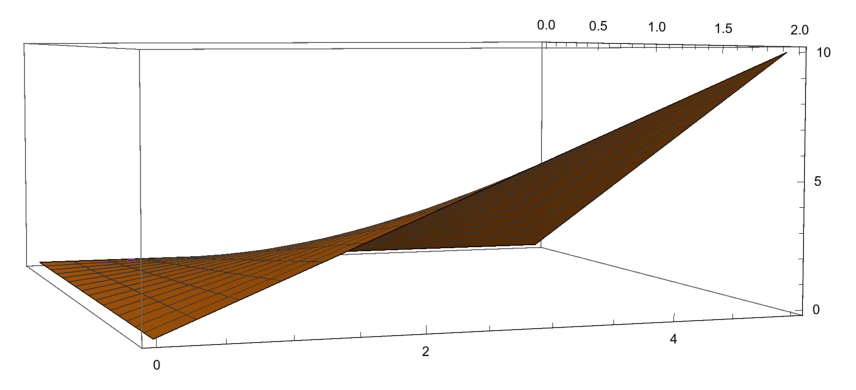
\epsfig{file=xy.eps, scale=.3}

The function $f(x, y)=xy$ and the constraint $y={{10-5x}\over{2}}$

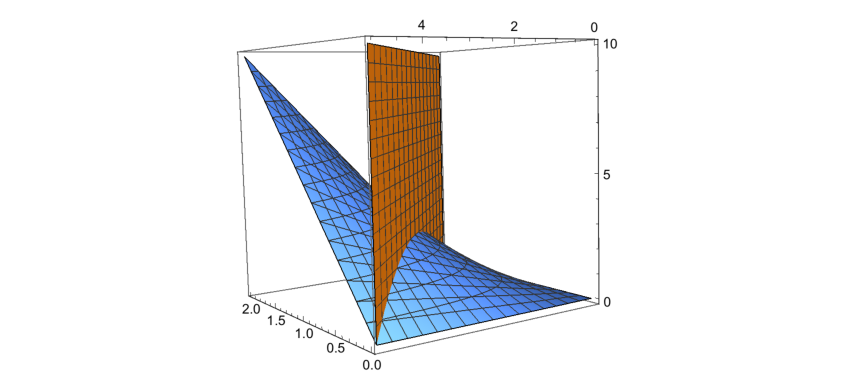
\epsfig{file=xyConst.eps, scale=.6} %Note to self: Use ContourPlot3D to make picture
\end{center}

\end{frame}


\begin{frame}
The method of Lagrange multipliers will find all constrained maxima \textit{and} minima, so you need to be careful to check your solutions \\(Question: Why didn't our last example find a constrained \textit{minimum}?)

Example: Maximize $5x+y$ subject to $x^2+y^2=10$

$$L(x, y, \lambda)=5x+y-\lambda(x^2+y^2-10)$$

$$\nabla L=\begin{bmatrix}
5-2\lambda x\\
1-2 \lambda y\\
-x^2-y^2+10
\end{bmatrix} =\mathbf{0}$$

Solving for $x, y, \lambda$: $x={5\over 2\lambda}$, $y={1\over 2\lambda}$, $${{25}\over{4\lambda^2}}+{{1}\over{4\lambda^2}}-10=0 $$ and so $\lambda =\pm 0.851$  and $(x, y)=(2.93, 0.58)$ and $(-2.93, -0.58)$



\end{frame}


\begin{frame}
Maximize $5x+y$  subject to $x^2+y^2=10$

\ \\ $(x, y)=(2.93, 0.58)$ is our max $(-2.93, -0.58)$ is our min 

%Think about where the y-intercept is on the two lines that are in the figure!  They give us the highest and lowest intercepts
\begin{center}
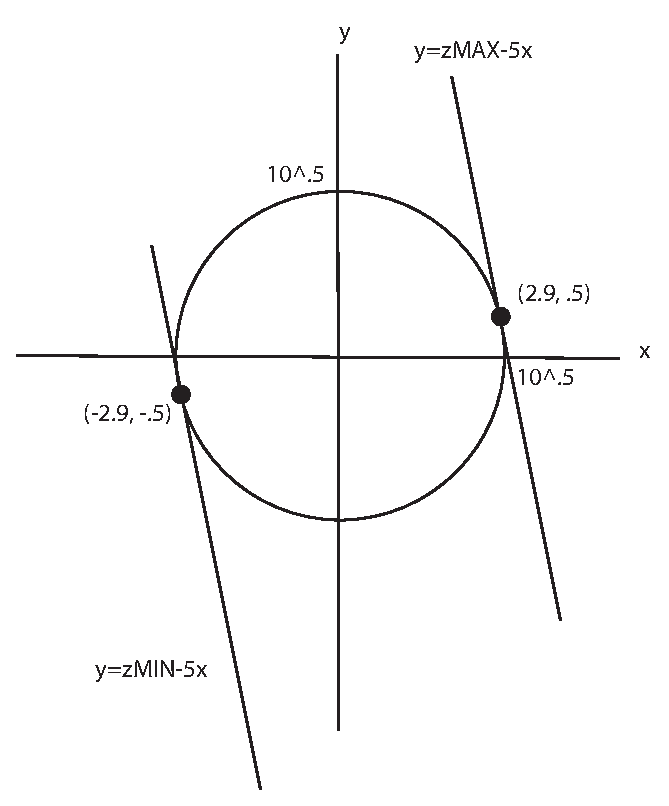
\epsfig{file=line.eps, scale=.45}
\end{center}
\end{frame}



\begin{frame}{Warnings}


\begin{itemize}
\item If your constraint isn't really a constraint, $L$ won't find it
\item Method provides a \textit{necessary} but not \textit{sufficient} condition for optima
\item A constrained optimum will be a critical point of the Lagrangian, but \textit{not necessarily a local maximum of the Lagrangian} (i.e. it could be a saddle of $L$)
\item With one constraint, the gradient of the constraint at an optimum can't equal $\mathbf{0}$ 
\end{itemize}
\end{frame}

\begin{frame}{What is $\lambda$?}


\ \\Consider a slightly different problem where we maximize $f(x, y)$ subject to $g(x, y)=b$, with $b$ a constant

\ \\The maximum value that $f$ can attain will generally depend on $b$; call this maximum value $v(b)$

\ \\If $(x^*, y^*)$ is a constrained maximum of $f$  with corresponding $\lambda$, then $\lambda=v^\prime(b)$

\ \\In words, $\lambda$ is the rate of change of the quantity being optimized as a function of the constraint parameter $b$.  Economically, it is how much you would pay to loosen the budget constraint.
\end{frame}
% Nice explanation on Khan academy website; it's a little complicated

\begin{frame}{More variables and more constraints}

\ \\If we have more than one constraint we create our Lagrangian with a different multiplier for each constraint (though we can't have more constraints than variables)

\ \\If we have more than two variables we simply take more first-order conditions to find our critical points

\begin{itemize}
\item \underline{Potential problem}: It's harder to characterize our critical points because we can't draw them out! 
\end{itemize}

\end{frame}

\begin{frame}{Concavity and Maxima}


\ \\Suppose that $f(\mathbf{x})$ is a concave function, that $g(\mathbf{x}), h(\mathbf{x}), ... $ are linear, and that we want to maximize $f$ subject to $g, h, ...$

\ \\Then if $L=f-\lambda(g)-\mu(h)-...$ has a critical point at $\mathbf{x}^*$, $f$ attains a constrained (global) maximum at $\mathbf{x}^*$

\ \\This extends in the obvious way to convex $f$ and global minima

\ \\$\Rightarrow$ Convexity or concavity of the objective function along with linear constraints yields unambiguous critical points


\end{frame}
\begin{frame}{A final example:}
 Maximize $-x^2-2y^2-3z^2$ subject to $x+y=5$ and $2x+y+z=10$

$$L(x, y, z, \lambda, \mu)=-x^2-2y^2-3z^2-\lambda(x+y-5)-\mu(2x+y+z-10)$$

$$\nabla L=\begin{bmatrix}
-2x-\lambda-2\mu\\
-4y-\lambda-\mu\\
-6z-\mu\\
-x-y+5\\
-2x-y-z+10
\end{bmatrix} =\mathbf{0}$$

\end{frame}
\begin{frame}

$$\nabla L=\begin{bmatrix}
-2x-\lambda-2\mu\\
-4y-\lambda-\mu\\
-6z-\mu\\
-x-y+5\\
-2x-y-z+10
\end{bmatrix} =\mathbf{0}$$

Solving (5 linear equations in 5 unknowns; I used R) we get $$x= \frac{25}{6},y = \frac{5}{6},z= \frac{5}{6},\lambda= \frac{5}{3},\mu= -5$$

\ \\Since our objective function is concave and our constraints are linear we know that  $x^*= \frac{25}{6},y^* = \frac{5}{6},z^*= \frac{5}{6}$ is a constrained optimum 


\end{frame}
 

\begin{frame}

$$\nabla L=\begin{bmatrix}
-2x-\lambda-2\mu\\
-4y-\lambda-\mu\\
-6z-\mu\\
-x-y+5\\
-2x-y-z+10
\end{bmatrix} =\mathbf{0}$$

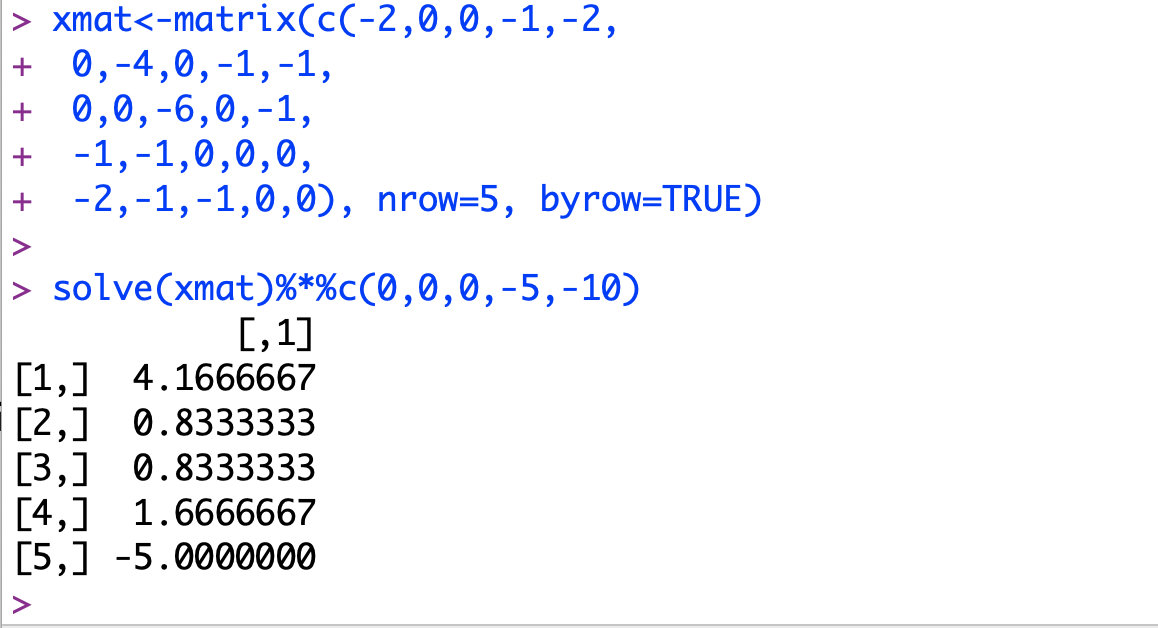
\includegraphics[width=3 in]{Rshot.png}

\end{frame}

\end{document}
